\documentclass[tikz]{standalone}
\usepackage{amsmath}
\definecolor{aksen}{RGB}{247,181,56}
\definecolor{bgdark}{HTML}{171D2B}
\begin{document}
\pagecolor{bgdark}
\color{white}
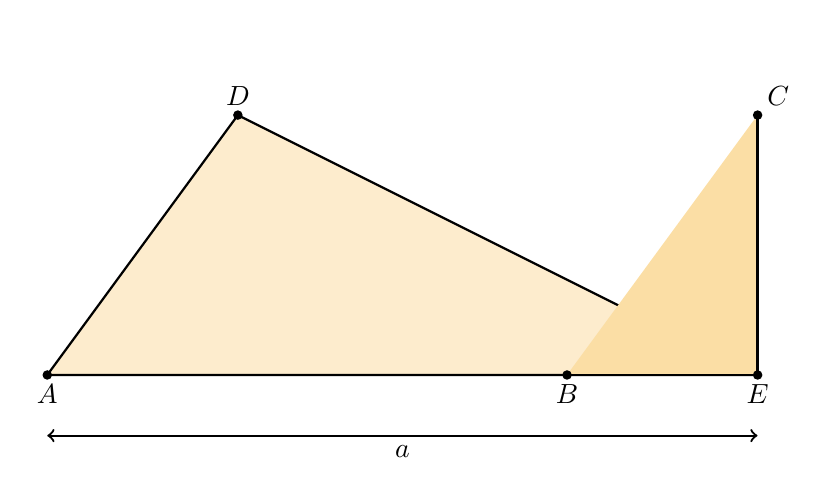
\begin{tikzpicture}[scale=1.1]
  % Panel 2: segitiga dipotong, digeser ke kanan, jadi persegi panjang
  \begin{scope}
    \coordinate (A) at (0,0);
    \coordinate (B) at (6,0);
    \coordinate (E) at (8.2,0);
    \coordinate (C) at (8.2,3);
    \coordinate (D) at (2.2,3);
    % bagian trapesium yang tersisa
    \fill[color=aksen!25] (A) -- (B) -- (E) -- (D) -- cycle;
    \draw[thick] (A) -- (B) -- (E) -- (D) -- cycle;
    % segitiga hasil geser: dari DH ke kanan
    \fill[color=aksen!45] (6,0) -- (8.2,0) -- (8.2,3) -- cycle;
    \draw[thick] (6,0) -- (8.2,0) -- (8.2,3);
    \draw[->,thick,white] (1.1,3.5) -- (5.5,3.5) node[midway,above] {digeser};
    \fill (D) circle (0.055) node[above] {$D$};
    \fill (A) circle (0.055) node[below] {$A$};
    \fill (B) circle (0.055) node[below] {$B$};
    \fill (E) circle (0.055) node[below] {$E$};
    \fill (C) circle (0.055) node[above right] {$C$};
    \draw[<->,thick] (0,-0.7) -- (8.2,-0.7) node[midway,below] {$a$};
  \end{scope}
\end{tikzpicture}
\end{document}
